%%%%%%%%%%%%%%%%%%%%%%%%%%%%%%%%%%%%%%%%%
% NIWeek 2014 Poster by T. Reveyrand
% www.microwave.fr
% http://www.microwave.fr/LaTeX.html
% ---------------------------------------
% 
% Original template created by:
% Brian Amberg (baposter@brian-amberg.de)
%
% This template has been downloaded from:
% http://www.LaTeXTemplates.com
%
% License:
% CC BY-NC-SA 3.0 (http://creativecommons.org/licenses/by-nc-sa/3.0/)
%
%%%%%%%%%%%%%%%%%%%%%%%%%%%%%%%%%%%%%%%%%

%----------------------------------------------------------------------------------------
%	PACKAGES AND OTHER DOCUMENT CONFIGURATIONS
%----------------------------------------------------------------------------------------

\documentclass[a0paper,portrait]{baposter}

\usepackage[font=small,labelfont=bf]{caption} % Required for specifying captions to tables and figures
\usepackage{booktabs} % Horizontal rules in tables
\usepackage{relsize} % Used for making text smaller in some places

\usepackage{amsmath,amsfonts,amssymb,amsthm} % Math packages
\usepackage{eqparbox}

\usepackage{textcomp}
\usepackage{multicol}
\usepackage{wrapfig} % Allows wrapping text around tables and figures

\usepackage{enumerate} % Customized item style
\usepackage{mdwlist} % Tight lists
\usepackage{threeparttable}
\usepackage{tcolorbox}
\usepackage{multirow}
\usepackage{setspace} % For 'spacing' environment


\renewcommand{\familydefault}{\sfdefault}

\graphicspath{{figures/}} % Directory in which figures are stored

 \definecolor{bordercol}{RGB}{40,40,40} % Border color of content boxes
 \definecolor{headercol1}{RGB}{186,215,230} % Background color for the header in the content boxes (left side)
 \definecolor{headercol2}{RGB}{120,120,120} % Background color for the header in the content boxes (right side)
 \definecolor{headerfontcol}{RGB}{0,0,0} % Text color for the header text in the content boxes
 \definecolor{boxcolor}{RGB}{210,235,250} % Background color for the content in the content boxes
 
 \definecolor{Mycolor1}{RGB}{160,183,210}
 \definecolor{Mycolor2}{RGB}{177,202,228}
 \definecolor{Mycolor3}{RGB}{255,255,255}



% Define a new command for text subscript
\newcommand{\tsub}{\textsubscript}

 \newcommand{\compresslist}{%
 \setlength{\itemsep}{0pt}%
 \setlength{\parskip}{0pt}%
 \setlength{\parsep}{0pt}%
 }
 
 \usepackage{enumitem}
\setlist[itemize]{noitemsep, topsep=0pt, leftmargin=1em}

\renewcommand\labelitemi{$\ast$}

\begin{document}

\begin{poster}{
grid=false,
borderColor=Mycolor1, % Border color of content boxes
headerColorOne=Mycolor2, % Background color for the header in the content boxes (left side)
headerColorTwo=Mycolor3, % Background color for the header in the content boxes (right side)
headerFontColor=headerfontcol, % Text color for the header text in the content boxes
%boxColorOne=boxcolor, % Background color for the content in the content boxes
headershape=roundedright, % Specify the rounded corner in the content box headers
headerfont=\Large\sf\bf, % Font modifiers for the text in the content box headers
textborder=faded,
background=none,
headerborder=open, % Change to closed for a line under the content box headers
boxshade=plain,
colspacing=0.6em,
headerheight=0.12\textheight
}
{
\includegraphics[height=30mm]{rsph.png}}
%
%----------------------------------------------------------------------------------------
%	TITLE AND AUTHOR NAME
%----------------------------------------------------------------------------------------
%
{ \bf  \LARGE {Incorporating Snow and Cloud Fractions in Random Forest to Estimate High-Resolution PM\tsub{2.5} Exposures in New York State} }
%\Large \it A} % Poster title
{\vspace{0.3em} \smaller Jianzhao Bi$^1$, Yujie Wang$^3$, Alexei Lyapustin$^3$, Avani Wildani$^2$, Yang Liu$^{1\ast}$\\  % Author names
\small $^1$\it {Environmental Health Sciences, Emory University , Atlanta, GA, United States} \\
\small $^2$\it {Department of Math and Computer Science, Emory University, Atlanta, GA, United States} \\
\small $^3$\it {Goddard Space Flight Center, NASA, Greenbelt, MD, United States}
}
{
\includegraphics[height=25mm]{logo.png}} 

%----------------------------------------------------------------------------------------
%	Background
%----------------------------------------------------------------------------------------
\headerbox{Background}{name=abstract,column=0,row=0,span=3}{
\begin{minipage}{0.76\textwidth}
Satellite aerosol optical depth (AOD) has been extensively utilized to predict ground-level fine particle (PM\tsub{2.5}) concentrations. However, 1) snow and cloud covers have led to a large proportion of non-random missing AOD observations, and 2) they can also lead to the change of the AOD level because of the shifted aerosol physical characteristics under different meteorological conditions (aerosol hygroscopic growth). Among the current approaches to address the AOD data gap issue, few have considered the cloud-AOD relationship and none of them have considered the snow-AOD relationship, which may lead to biases in PM\tsub{2.5} prediction. In this study, we incorporated satellite-retrieved snow and cloud fractions into a gap-filling model to estimate missing AOD under the extensive cloud and snow covers. Based on the gap-filled AOD, fully covered PM\tsub{2.5} predictions with a 1-km resolution were generated.
\end{minipage}
\hspace{3pt}
\begin{minipage}{0.22\textwidth}
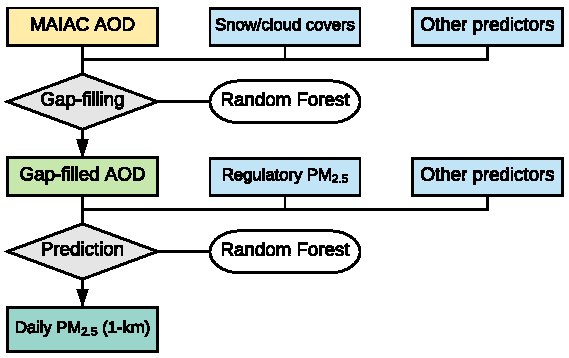
\includegraphics[width=\textwidth]{steps.pdf}
\end{minipage}

}

%----------------------------------------------------------------------------------------
%	AOD Gap-filling
%----------------------------------------------------------------------------------------
\headerbox{AOD Gap-filling}{name=instruments,column=1,row=1,span=2,below=abstract}
{
\begin{minipage}{0.6\textwidth}
\textbf{Table 2.} Satellite AOD missing rates in NYS in 2015

\begin{threeparttable}
\begin{tabular}{p{0.2\textwidth}<{\centering}p{0.13\textwidth}<{\centering}p{0.13\textwidth}<{\centering}p{0.32\textwidth}<{\centering}}
    \toprule
    \footnotesize\textbf{Missing Type} & \footnotesize\textbf{Mean} & \footnotesize\textbf{Median} & \footnotesize\textbf{25$^{th}$ -- 75$^{th}$ Quantiles} \\
    \midrule
    Overall & 90.27\% & 96.54\% & 87.62\% -- 99.84\% \\
    Cloud & 75.58\% & 79.47\% & 64.74\% -- 91.48\% \\
    Snow & 6.14\% & 0\% & 0\% -- 2.48\% \\
    Snow season\tnote{1} & 21.15\% & 14.03\% & 5.23\% -- 31.18\% \\
    \bottomrule
\end{tabular}
\begin{tablenotes}
\footnotesize
\item [1] Snow season is the first 15 weeks of 2015 in NYS
\end{tablenotes}
\end{threeparttable}
\end{minipage}
\begin{minipage}{0.38\textwidth}
\begin{itemize}
\compresslist
    \item The quality assessment flags of MAIAC were used to infer the missing AOD caused by cloud/snow covers
    \item As the majority of missing AOD caused by the snow cover occurred in the first 15 weeks of 2015, the missing rates in this period were separately summarized
\end{itemize}
\end{minipage}
        
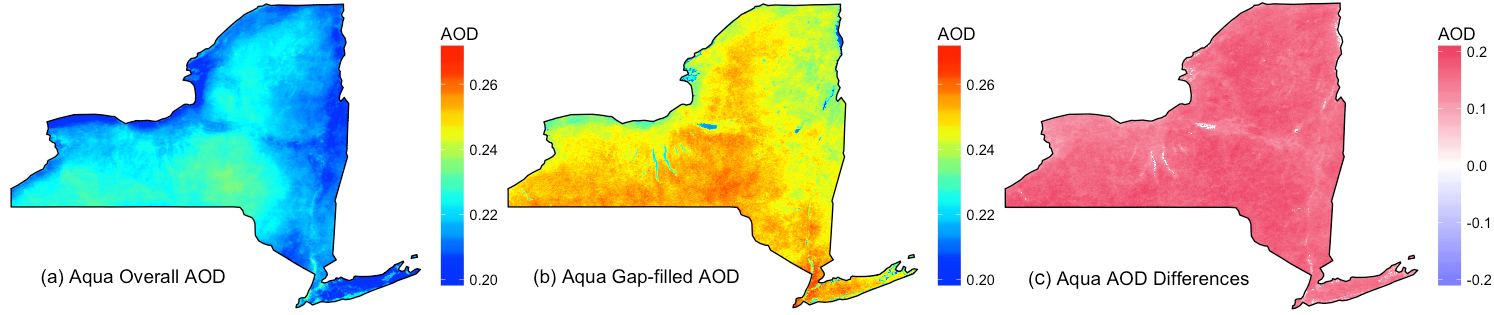
\includegraphics[width=\textwidth]{aod.jpg}
\small{
\textbf{Figure 3.} AOD spatial distributions in 2015: (a) the annual distribution of Aqua AOD; (b) the annual distribution of gap-filled Aqua AOD; (c) differences between gap-filled and original Aqua AOD.
}
\begin{itemize}
\compresslist
    \item In Fig. 3, original and gap-filled AOD had annual means of 0.09 (IQR: [0.08, 0.10]) and 0.25 (IQR: [0.24, 0.25]), respectively. 
    \item The gap-filled AOD was higher than the original AOD throughout the state (Fig. 3(c)), which agreed with previous studies who found clear evidence that the hygroscopic growth of aerosol droplets under cloudy and humid weather led to higher levels of AOD.
\end{itemize}

}

%----------------------------------------------------------------------------------------
%	Data and Methods
%----------------------------------------------------------------------------------------
\headerbox{Data and Methods}{name=calibration,column=0,row=1,below=abstract}
{
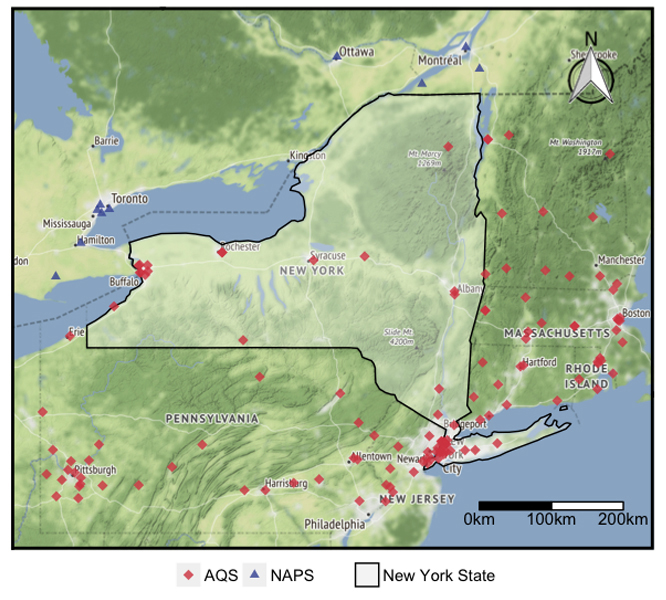
\includegraphics[width = \textwidth, height = 0.85\textwidth]{ny.jpg}
\small{\textbf{Figure 1.} Study domain included New York State and its surrounding areas (used as the buffer). Red diamonds are EPA AQS stations. Blue triangles are NAPS stations. The time period of this study was 2015.}

\vspace{0.3em}
\begin{tcolorbox}[boxsep=0pt,left=3pt,right=3pt]
\centering\textbf{AOD Gap-filling Model}
\linespread{0.8}\selectfont
\begin{align*}
\mathrm{AOD_{\mathit{st}}=}&\mathrm{f(Snow/Cloud\;Frac_{\mathit{st}}, Meteorological_{\mathit{st}},}\\
    &\mathrm{Elevation_\mathit{s}, Spatial\;Coord_\mathit{s})}
\end{align*}
\centering\textbf{PM\tsub{2.5} Prediction Model}
\begin{align*}
    \mathrm{PM}&\mathrm{_{2.5\mathit{st}}=f(\operatorname{Gap-filled}\;AOD_{\mathit{st}},PM_{2.5}\;Cov_{\mathit{st}},}\\
    &\mathrm{Meteorological_{\mathit{st}},Landuse_\mathit{s},Month_\mathit{t}, Day_\mathit{t})}
\end{align*}
\end{tcolorbox}
\vspace{0.3em}

\textbf{Table 1.} Model performance

\begin{threeparttable}
    \begin{tabular}{p{0.32\textwidth}<{\centering}p{0.32\textwidth}<{\centering}p{0.18\textwidth}<{\centering}}
        \toprule
        \textbf{Model} & \textbf{Algorithm} & \textbf{CV R$^2$} \\
        \midrule
        AOD Gap-filling & \multirow{2}{*}{Random Forest} & 0.93 \\
        PM\tsub{2.5} Prediction & & 0.82 \\
        \bottomrule
    \end{tabular}
\end{threeparttable}

\vspace{0.95em}
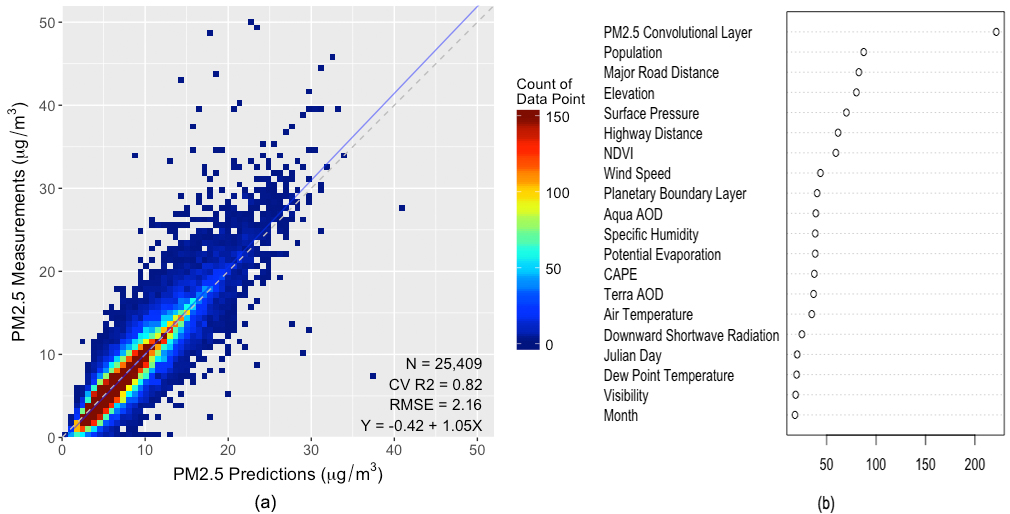
\includegraphics[width=\textwidth]{rf.jpg}
\small{
\textbf{Figure 2.} PM\tsub{2.5} prediction model performance: (a) 10-fold cross-validation (CV) scatters with an R$^2$ of 0.82 and an RMSE of 2.16 $\mu g/m^3$; (b) variable importance ranking in which the PM\tsub{2.5} convolutional layer had the highest value and five of the top-seven important variables were land-use variables.
}

}

%----------------------------------------------------------------------------------------
%	PM2.5 Prediction
%----------------------------------------------------------------------------------------
\headerbox{PM\tsub{2.5} Prediction}{name=receiver,span=2,column=1,row=1, below=instruments}{

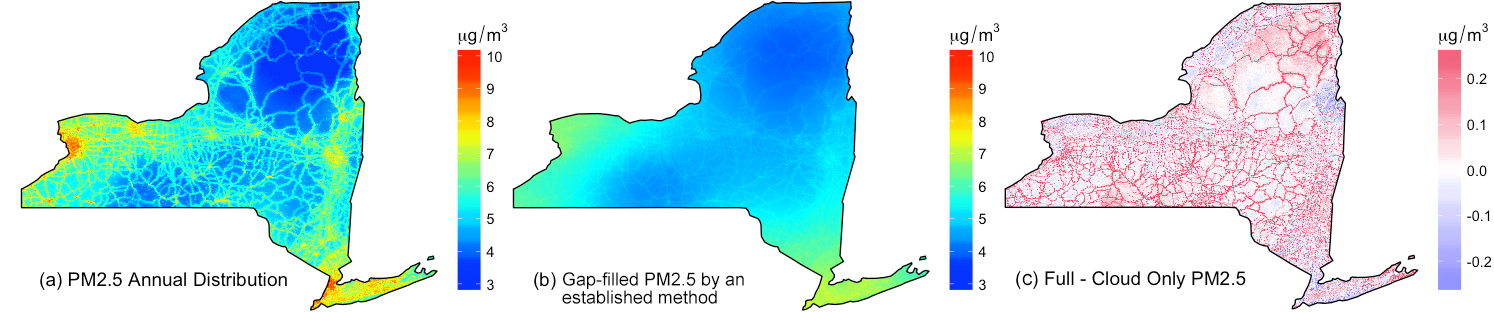
\includegraphics[width=\textwidth]{pm25.jpg}
\small{\textbf{Figure 4.} PM\tsub{2.5} spatial distributions in 2015: (a) the annual distribution of PM\tsub{2.5} with a 1-km resolution; the mean concentration was 5.30 $\mu g/m^3$ (IQR: 4.43 to 6.08 $\mu g/m^3$) (b) the annual distribution of PM\tsub{2.5} by an established gap-filled method, which appeared to over-smooth the PM\tsub{2.5} spatial details; (c) differences between full-model and cloud-only PM\tsub{2.5} in the snow season.}

\vspace{5pt}

\begin{minipage}{0.345\textwidth}
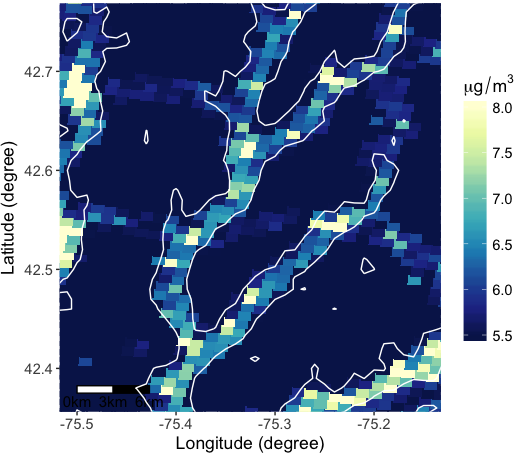
\includegraphics[width=\textwidth]{valley.png}
\end{minipage}
\begin{minipage}{0.655\textwidth}
\begin{itemize}
\compresslist\small
    \item In Fig. 4(a), higher PM\tsub{2.5} levels were along with the roads and in the populated areas, which agreed with the PM\tsub{2.5} emission inventory of NYS (NEI 2014). 
    \item By adding the snow parameter to the AOD gap-filling model, PM\tsub{2.5} concentrations changed by an absolute mean of 0.09 $\mu g/m^3$ with a maximum of 0.99 $\mu g/m^3$ (Fig. 4(c)), showing the importance of this parameter in the model.
    \item In Fig. 5, the PM\tsub{2.5} concentrations in the valleys were $\sim$1--2 $\mu g/m^3$ higher than which in the surroundings, indicating that our product was able to reflect small-scale PM\tsub{2.5} features driven by local geographical factors.
\end{itemize}
\small{\textbf{Figure 5.} PM\tsub{2.5} with contours in a valley area of Upstate New York, showing the PM\tsub{2.5} accumulation effect in the valleys in winter}
\end{minipage}
}

%----------------------------------------------------------------------------------------
%	CONCLUSION
%----------------------------------------------------------------------------------------
\headerbox{Conclusion}{name=conclusion,column=1,below=receiver,above=bottom,span=2}
{
\begin{spacing}{0.9}
\small{
By incorporating the snow/cloud fractions into the gap-filling process, a 100\% gap-filled AOD dataset was produced with good model performance. The 1-km PM\tsub{2.5} predictions derived from the gap-filled AOD were able to reflect detailed emission patterns and small-scale terrain-driven features. Although we only applied fraction measures of snow and cloud, the importance of these parameters was still reflected and the discernible interactions between snow/cloud and AOD/PM\tsub{2.5} were observed. The methodology of this study can be generalized to other areas with extensive snow/cloud covers and large proportions of missing satellite AOD data to estimate PM\tsub{2.5} exposures which could not be obtained before.
}
\end{spacing}
}
%----------------------------------------------------------------------------------------
%	REFERENCES
%----------------------------------------------------------------------------------------
%\headerbox{References}{name=references,column=1,below=conclusion,span=2}{

%}
%----------------------------------------------------------------------------------------
%	ACKNOWLEDGEMENTS
%----------------------------------------------------------------------------------------
\headerbox{Acknowledgements}{name=acknowledgements,column=0,row=2,below=calibration, above=bottom}{
\begin{spacing}{0.9}
\small{The work of J. Bi and Y. Liu is supported by the NASA Applied Sciences Program (Grant \# NNX14AG01G and NNX16AQ28G, PI: Liu) and the National Institute of Environmental Health Sciences of the National Institutes of Health under Award Number P30ES019776. Please direct your questions to Prof. Yang Liu (yang.liu@emory.edu).}
\end{spacing}

} 
\end{poster}
\end{document}